\section{Web Gallery Prototype}
\subsection{Zusammenfassung [M]} 
\setauthor{Fabian Maar}
In diesem Abschnitt wird erklärt, auf welche Weise die 3D-Ausstellung in der Webapplikation realisiert wurde. Dabei wurde das Konzept des evolutionären Prototypings (siehe Prototyping \ref{ch::ongoing-prototyping}) für die Entwicklung verwendet. 

\subsection{Rendering [M]} 
Um 3D-Modelle, wie den Ausstellungsraum anzeigen zu können, wird der hochkomplexe Prozess des Renderings benötigt. Dabei wird das 3D-Modell zu einem realistischen 2D-Bild gerendert. 
\cite{AdobeRendering} \cite{Rendering3DModels}

\subsubsection{Der Prozess des Renderings}
Hinter dem Rendering stecken verschiedene Algorithmen, die ein solches 3D Modell anzeigen lassen. Verschiedene Werte und Daten werden zur Berechnung benötigt, welche die Qualität und die Geschwindigkeit des Prozesses unterschiedlich beeinflussen:

\begin{itemize}
    \item das 3D-Objekt und wie realistisch es dargestellt werden soll
    \item die Art des Renderns
    \item die Lichtquellen und die entstehenden Schatten; wird Behandel im Kapitel Lichtsetzung \ref{lichtsetzung}
    \item die Kameraposition und Renderbereich (Clipping)
    \item der Anti-aliasing Prozess
    \item die Art des Render-Algorithmuses
    \item weitere atmosphärische Effekte 
    
    
\end{itemize}
\cite{Rendering3DModels}

\subsubsection{3D-Modelle}
3D-Modelle besitzen verschiedene Eigenschaften, wie zum Beispiel ihre Textur, Farbe oder ihre Fähigkeit Licht zu reflektieren, die beim Rendern berücksichtigt werden müssen. Die 3D-Daten des Modells werden ermittelt und dabei in Pixelinformationen umgewandelt. Diese werden durch die Ermittlung der Koordinaten des Objektes an bestimmten Positionen abgebildet. \cite{Rendering3DModels}

\subsubsection{Arten des Renderns}
Beim Rendern wird zwischen folgenden Arten unterscheiden:

\begin{itemize}
    \item Offline-Rendering - Das Offline-Rendering rendert über einen längeren Zeitraum in hoher und realistischer Qualität. Diese Art kommt zum Beispiel bei Filmen zum Einsatz. 
    \item Echtzeit-Rendering - Beim Echtzeit-Rendering wird ein 3D-Modell in kürzester Zeit gerendert. Diese Art kommt zum Beispiel bei Videospielen oder im 3D-Gallery zum Einsatz. Hierbei werden meist 24 Bilder pro Sekunde gerendert, um Bewegungen flüssig wahrzunehmen. 
\end{itemize}
\cite{RenderArten}

\subsubsection{Clipping}
\label{clipping}
Beim Clipping werden Ebenen zur Begrenzung des Bereichs, den es zu rendern gilt, erstellt. Diese Ebenen werden durch die Weltkoordinaten positioniert. Die seitlichen sowie die unteren und oberen Clipping-Ebenen werden durch die Kameraposition und die Fensterposition definiert. Auch gibt es das Far- und Near-Clipping, wodurch zum einen die Tiefe des 3D-Modells begrenzt wird. Zum anderen werden unerwünschte Objekte, die im Hintergrund liegen, ebenfalls nicht gerendert. \cite{Rendering3DModels}


\subsubsection{Anti-Aliasing}
Beim Anti-Aliasing Prozess wird versucht, den auftretenden Aliasing-Effekt zu reduzieren und zu entfernen. Der Aliasing-Effekt tritt auf, wenn die Pixel zu grob für feine Strukturen und Muster sind. Der Effekt ist besonders stark, wenn diese Muster nicht senkrecht sind. Dieser Aliasing-Effekt wirkt sich auf das 3-Modell aus, in dem Zacken an Polygon-Kanten entstehen, ein Moiré-Effekt auftritt ( siehe Abbildung \ref{fig:impl:MoireEffekt}) Verweis oder generell unerwünschte Muster auftreten.\cite{Rendering3DModels} 
\begin{figure}
    \centering
    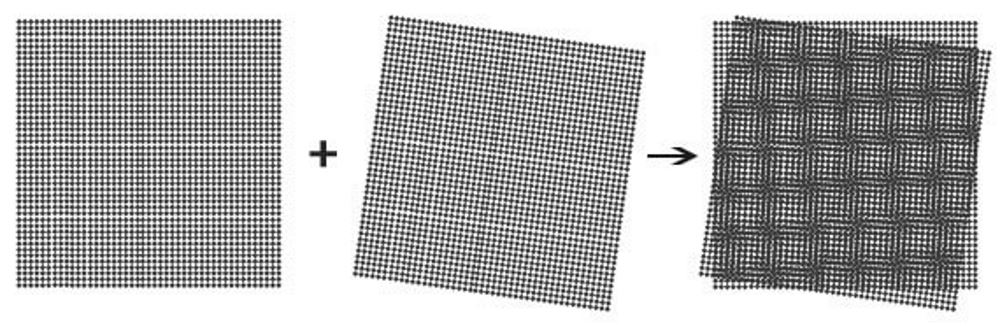
\includegraphics[scale=0.3]{pics/moire-effekt.jpg}
    \caption{Der Moire-Effekt visualisiert \cite{MoireEffekt}}
    \label{fig:impl:MoireEffekt}
\end{figure}

\begin{figure}
    \centering
    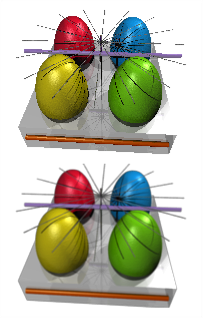
\includegraphics[scale=0.7]{pics/anti-aliasing.png}
    \caption{Rendering mit und ohne Anti-Aliasing \cite{AntiAliasing}}
    \label{fig:impl:anti-aliasing}
\end{figure}

\subsubsection{Verschiedene Render-Algorithmen [M]}
\subsubsection{Rasterization}
Über den Bildschirm wird ein Raster aus meistens Dreiecken gespannt, da diese am einfachsten zu berechnen sind. In den Ecken der Dreiecke, auch genannt Scheitelpunkte, sind die Informationen enthalten, die zur Darstellung eines 3D-Objektes in 2D benötigt werden. Dieser Prozess wird für Echtzeit-Rendering genutzt. Er ist zwar rechenintensiv, jedoch nicht so intensiv wie beim Ray-Tracing. \cite{RayTracingRasterization}

\subsubsection{Wire-Frame}
Bei einem Wire-Frame wird ein 3D-Modell erstellt, in dem der Algorithmus versucht, lineare Merkmale wie Kanten oder Konturlinien zu verfolgen. Dabei werden auch verdeckte oder nicht-sichtbare Teile inkludiert. 
\cite{Rendering3DModels} 

\subsubsection{Visible Line}
Dieser Vorgang funktioniert ähnlich wie ein Wire-Frame, nur dass hierbei nur Linien gerendert werden, die tatsächlich von der Kamera sichtbar sind. Dieser sichtbare Bereich wird auch Visible Surface genannt. 
\cite{Rendering3DModels} 

\subsubsection{Raycasting}
\label{impl:rend:raycasting}
Beim Raycasting wird ermittelt, welches 3D-Objekt zuerst von einem Ray getroffen wird. Ein Ray ist ein Strahl, der von der Position der Kamera ausgeht. Für jedes Pixel wird ein Ray durch den dreidimensionalen Raum geschickt. Dadurch können die Schnittpunkte der Objekte und der Rays ermittelt werden. Dabei werden alle Objekte mit einem sichtbaren Schnittpunkt angezeigt und die Fläche normal dazu bestimmt die Schattierung. Dieser Prozess wird im Kapitel \ref{impl:int:raycasting} näher erklärt und angewandt.
\cite{Rendering3DModels} 

\subsubsection{Ray-Tracing}
Der Ray-Tracing Prozess funktioniert ähnlich wie der Prozess des Raycastings. Beim Ray-Tracing werden jedoch auch verschiedene Oberflächen und Lichtquellen berücksichtigt. Dies funktioniert, indem ein Ray vom Algorithmus mitverfolgt wird. Dabei ist es möglich, zu erkennen ob ein Ray:
\begin{itemize}
    \item durch eine lichtdurchlässige Oberfläche durchdringt
    \item von einem reflektierenden Objekt reflektiert wird
    \item oder ob ein Objekt von einer Lichtquelle getroffen wird und einen Schatten wirft
\end{itemize}
\cite{RayTracingRasterization}

\begin{figure} [h]
    \centering
    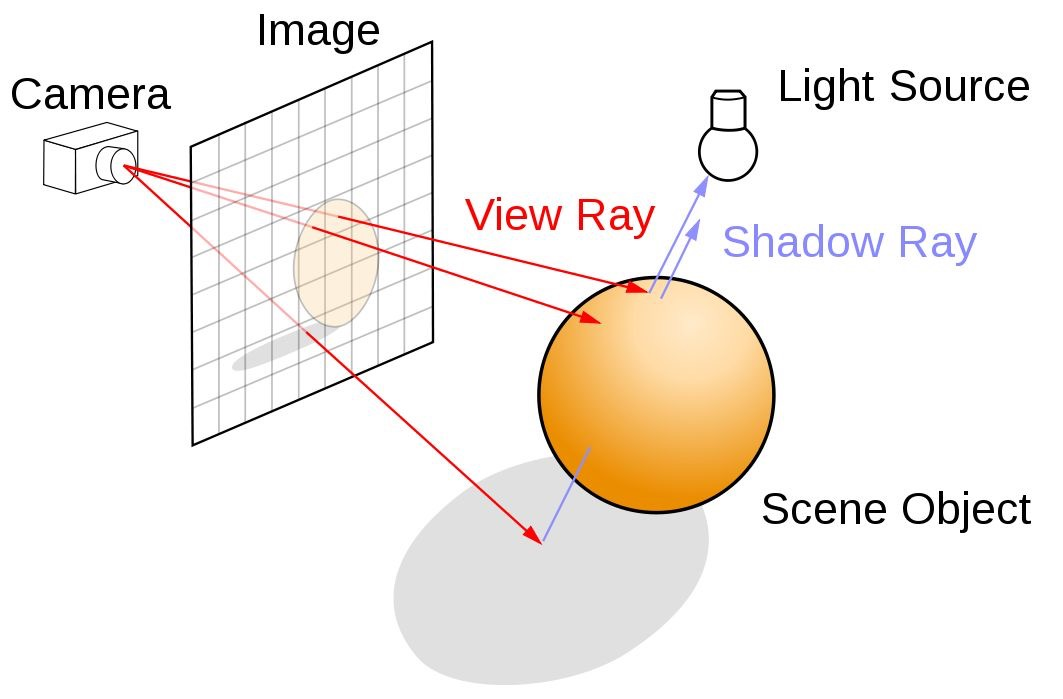
\includegraphics[scale=0.3]{pics/ray-tracing.jpg}
    \caption{Vorgang des Ray-Tracing \cite{RayTracingRasterization}}
    \label{fig:impl:ray-tracing}
\end{figure}


\subsubsection{Rendering in Three.js}
Für das Rendern der 3D-Gallery wird der in Three.js inkludierte Renderer von WebGL (siehe ThreeJS \ref{ch::webgl}) Referenz verwendet. Um das gerenderte 3D-Objekt in das DOM (siehe DOM \ref{txt:glos:API}) zu integrieren, wird das HTML-Element <canvas> verwendet. \cite{ThreejsWebGLRenderer}

\begin{lstlisting}[caption={Canvas-Element in HTML},language=HTML,label=lst:impl:canvas]
    <canvas #threeCanvas style="width: 100%;  height: 100%" (window:resize)="onResize($event)"></canvas>
\end{lstlisting}
Dabei wird dieses DOM-Element als Angular-View-Child initialisiert. Dadurch können Änderungen am Dom erkannt und das betroffene Element neu definiert werden. \cite{AngularViewChild}
\begin{lstlisting}[caption={Canvas als View-Child initialisieren},language=TypeScript,label=lst:impl:viewchild]
    @ViewChild('threeCanvas') threeCanvas!: ElementRef;
\end{lstlisting}
Anschließend wird ein neuer WebGLRenderer angelegt, dem der Canvas zugewiesen wird. Falls noch kein Canvas besteht, wird automatisch ein neuer erstellt. \cite{ThreejsWebGLRenderer}
\begin{lstlisting}[caption={WebGlRenderer anlegen},language=TypeScript,label=lst:impl:WebGlRenderer]
    this.renderer = new THREE.WebGLRenderer({
        canvas: this.threeCanvas.nativeElement
      });
\end{lstlisting}
Um die Render-Funktion des Renderers als Echtzeit-Rendering anzuwenden, wird eine Render-Schleife benutzt. Darin ist zum einen die Render-Funktion mit der Szene und der Kamera, die gerendert werden soll. In einer Szene befinden sich alle 3D-Objekte. Zum anderen befindet sich die Funktion requestAnimationFrame in der Schleife, wodurch die Szene jedes Mal neu gerendert wird, wenn der Bildschirm neu geladen wird. Dies geschieht üblicherweise 60-mal in der Sekunde. \cite{ThreejsCreateAScene}
\begin{lstlisting}[caption={Animations-Schleife},language=TypeScript,label=lst:impl:animationloop]
    animate = () => {
        requestAnimationFrame(this.animate);
        this.renderer.render(this.scene, this.camera!)
    }  
\end{lstlisting}
\subsection{Resizing [L]} 
\setauthor{Litzlbauer Lorenz}
https://www.omnicalculator.com/other/resolution-scale
https://discourse.threejs.org/t/render-half-size-then-upscale/13228

\subsection{Lichtsetzung}
\label{lichtsetzung}
Das Licht ist das 2. Wichtig, denn ohne würden die gerenderten Objekte im Dunklen stehen. Um dies zu ändern, wird eine Lichtquelle installiert, um einen bestimmten Bereich der Szene zu erhellen. Dabei können ebenfalls unterschiedliche Optionen konfiguriert werden, um die Szene so realistisch wie möglich aussehen zu lassen. Das Licht wird jedoch nicht nur von der Lichtquelle beeinflusst, sondern auch von dem Objekt, das beleuchtet wird. Material und Oberfläche eines Objektes reagieren unterschiedlich auf den Einfall des Lichtes, wodurch zum Beispiel die Lichtreflektion stärker ausfällt. Dieses Konzept wird auch Global Illumination genannt. Three.js bietet eine Vielzahl von Lichtarten und Quellen:

\begin{itemize}
    \item Das Standard-Licht, Light genannt, ist das Grundgerüst der anderen Lichttypen. Es kann die Farbe und Intensität des Lichtes individuell geändert werden. \cite{StandardLight}
    \item Die LightProbe ist eine alternative Methode, Licht zu erzeugen. Dabei wird nicht direkt von einer Quelle das Licht ausgestrahlt, sondern es speichert die Lichtinformation ab. Dabei wird erst beim Rendern der Lichteinfall durch die Daten der LightProbe ermittelt.  \cite{LightProbe}
    \item Das AmbientLight belichtet die gesamte Szene gleich, kann dabei jedoch keine Schatten werfen. \cite{AmbientLight}
    \item Das DirectionalLight wirft Licht parallel in eine bestimmte Richtung. Da es unendlich weit weg erscheint, wird es oft als Tages- oder Sonnenlicht verwendet. \cite{DirectionalLight}
    \item Das HemisphereLight wird über der Szene positioniert und besitzt eine Himmel- und Bodenfarbe mit Verlauf. Diese Lichtquelle kann keine Schatten werfen \cite{HemisphereLight}
    \item Das PointLight wirft Licht von einem Punkt in alle Richtungen. Es soll eine Glühbirne simulieren. Hierbei kann ebenfalls die Reichweite des Lichtes und ein Dimmeffekt bestimmt werden. \cite{PointLight}
    \item Das RectAreaLight strahlt Licht in Form eines Rechtecks aus. Damit können zum Beispiel Fenster simuliert werden \cite{ReactAreaLight}
    \item Das SpotLight wirft Licht in Form eines Kegel \cite{SpotLight}
\end{itemize}

Das Point Light wurde in der 3D-Ausstellung wie folgt angewandt:  
\begin{lstlisting}[caption={Lichtsetzung in der 3D-Ausstellung},language=TypeScript,label=lst:impl:pointlight]
    const bulbGeometry = new THREE.SphereGeometry(.02, 16, 8);
    const bulbLight = new THREE.PointLight( 0xffffff, 3, 1000, 2); 
    const bulbMat = new THREE.MeshStandardMaterial( {
          emissive: 0xffffff,
          emissiveIntensity: 1,
          color: 0x000000
        } );
        bulbLight.add( new THREE.Mesh( bulbGeometry, bulbMat ) );
        bulbLight.position.set( 0, 100, 0 );
        bulbLight.castShadow = true;
        this.scene.add( bulbLight );
\end{lstlisting}
Zunächst wurde ein Objekt angelegt, welches das Licht ausstrahlen soll. Anschließend wird die Lichtquelle und deren Material initialisiert. Um Schatten zu werfen, wird das Attribut .castShadow auf true gesetzt. 

